\documentclass{article}

\usepackage[utf8]{inputenc}
\usepackage[russian]{babel}
\usepackage[a4paper, margin=1in]{geometry}
\usepackage{graphicx}
\usepackage{amsmath}
\usepackage{wrapfig}
\usepackage{multirow}
\usepackage{mathtools}
\usepackage{pgfplots}
\usepackage{pgfplotstable}
\usepackage{setspace}
\usepackage{changepage}
\usepackage{caption}
\usepackage{csquotes}
\usepackage{hyperref}
\usepackage{listings}

\pgfplotsset{compat=1.18}
\hypersetup{
  colorlinks = true,
  linkcolor  = blue,
  filecolor  = magenta,      
  urlcolor   = darkgray,
  pdftitle   = {
    math-tool-report-approx-smirnov-victor-p32131
  },
}

\definecolor{codegreen}{rgb}{0,0.6,0}
\definecolor{codegray}{rgb}{0.5,0.5,0.5}
\definecolor{codepurple}{rgb}{0.58,0,0.82}
\definecolor{backcolour}{rgb}{0.99,0.99,0.99}

\lstdefinestyle{codestyle}{
  backgroundcolor=\color{backcolour},   
  commentstyle=\color{codegreen},
  keywordstyle=\color{magenta},
  numberstyle=\tiny\color{codegray},
  stringstyle=\color{codepurple},
  basicstyle=\ttfamily\footnotesize,
  breakatwhitespace=false,         
  breaklines=true,                 
  captionpos=b,                    
  keepspaces=true,                 
  numbers=left,                    
  numbersep=5pt,                  
  showspaces=false,                
  showstringspaces=false,
  showtabs=false,                  
  tabsize=2
}

\lstset{style=codestyle}

\begin{document}

\begin{titlepage}
    \begin{center}
        \begin{spacing}{1.4}
            \large{Университет ИТМО} \\
            \large{Факультет программной инженерии и компьютерной техники} \\
        \end{spacing}
        \vfill
        \textbf{
            \huge{Вычислительная математика.} \\
            \huge{Лабораторная работа №6.} \\
            \huge{
                Численное решение обыкновенных
                дифференциальных уравнений
            } \\
        }
    \end{center}
    \vfill
    \begin{center}
        \begin{tabular}{r l}
            Группа:  & P32131                  \\
            Студент: & Смирнов Виктор Игоревич \\
            Вариант: & 16                      \\
        \end{tabular}
    \end{center}
    \vfill
    \begin{center}
        \begin{large}
            2023
        \end{large}
    \end{center}
\end{titlepage}

\section*{Ключевые слова}
Дифференциальные Уравнения, Численные Методы.

\tableofcontents

\section{Цель работы}

Цель работы - решить задачу Коши для обыкновенных
дифференциальных уравнений численными методами.

\section{Используемые методы}

\subsection{Метод Эйлера}

Пусть дана Задача Коши для уравнения первого порядка.

\begin{equation}
    \frac{dy}{dx} = f(x, y), \; y(x_0) = y_0
\end{equation}

Хотим решить данной уравнение на интервале $[x_0, x_n]$,
который разобъем на интервалы с шагом $h$.

Тогда рабочая формула форумула метода будет:

\begin{equation}
    y_i = y_{i-1} + (x_i - x_{i-1})f(x_{i-1}, y_{i-1})
\end{equation}

Факты:
\begin{enumerate}
    \item Прост в реализации
    \item Имеет погрешность $O(h)$
\end{enumerate}

Также можно улучшить точность алгоритма, 
рассмотрев частный случай неявного метода Рунге — Кутты 
первого порядка:

\begin{equation}
    y^{'}_{n+1} = y_n + hf(x_n, y_n) - \text{Прогноз}
\end{equation}
\begin{equation}
    y_{n+1} = y_n + h \frac{f(x_n, y_n) + f(x_{n+1}, y^{'}_{n+1})}{2}
    - \text{Коррекция}
\end{equation}

\lstinputlisting[
    language={Python},
    caption={Реализация метода Эйлера на Python},
    linerange={11-57}
]{../src/diffeq/method/euler.py}


\subsection{Метод Рунге — Кутты 4ого порядка}

Задача аналогичная, метод другой.

Рабочая формула:

\begin{equation}
    k_1 = f(x_n, y_n)
\end{equation}
\begin{equation}
    k_2 = f(x_n + \frac{h}{2}, y_n + \frac{h}{2} k_1)
\end{equation}
\begin{equation}
    k_3 = f(x_n + \frac{h}{2}, y_n + \frac{h}{2} k_2)
\end{equation}
\begin{equation}
    k_3 = f(x_n + h, y_n + hk_3)
\end{equation}
\begin{equation}
    y_{n+1} = y_n + \frac{h}{6}(k_1 + 2k_2 + 2k_3 + k_4)
\end{equation}

Факты:
\begin{enumerate}
    \item Гораздо сложнее Эйлера
    \item Зато гарантирует погрешность $O(h^4)$
\end{enumerate}

\lstinputlisting[
    language={Python},
    caption={Реализация метода Рунге-Кутты на Python},
    linerange={11-64}
]{../src/diffeq/method/runge_kutta_4.py}


\subsection{Метод Милна}

Данный метод уже является многошаговым, то есть 
требует несколько точек для старта. Используется 
принцип прогноза и коррекции.

\begin{equation}
    y^{predict}_i = y_{i-4} + \frac{4h}{3}(2f_{i-3} - f_{i-2} + 2f_{i-1}), f_{i} = f(x_i, y_i)
\end{equation}
\begin{equation}
    f^{predict}_i = f(x_i, y^{predict}_i)
\end{equation}
\begin{equation}
    y^{correct}_i = y_{i-2} + \frac{h}{3}(f_{i-2} + 4f_{i-1} + f^{predict}_i)
\end{equation}

\lstinputlisting[
    language={Python},
    caption={Реализация метода Милне на Python},
    linerange={12-76}
]{../src/diffeq/method/milne.py}

\subsection{Правило Рунге}

Контроль точности осуществляется правилом Рунге.
\begin{equation}
    R = \frac{|y_i^h - y_i^{h/2}|}{2^p - 1} \leq \varepsilon
\end{equation}

\section{Примеры работы программы}

\begin{lstlisting}[
    language={Bash},
    caption={Результаты работы программы 0}
]
=== Welcome to differential eqsolver ===

Here you can solve differential equations using:
- Basic Euler
- Corrected Euler
- Runge-Kutta 4
- Milne

Choice a one of first-order equations:
[0]: dy/dx = y + (1 + x) * y ^ 2
[1]: dy/dx = -2 * y
[2]: dy/dx = 2 * x * exp(x ** 2) / (exp(x ** 2) + 1)
Enter a number of equation i in [0..2]: 0
Taken: dy/dx = y + (1 + x) * y ^ 2
Enter boundaties: 
Enter x_0: 1
Enter y_0: -1
Enter x_n: 1.5
Enter h: 0.1
Enter eps: 0.000001

Input parameters: 
> x_0 = 1.0
> y_0 = -1.0
> x_n = 1.5
> h   = 0.1
> eps = 1e-06

Enjoy results!

=== Report of Basic Euler === 

Result of Basic Euler is -0.6666664538724102
Total iterations: 327681
Stop at: 1.5000000000291038

=== Report of Corrected Euler === 

Result of Corrected Euler is -0.6666666666710818
Total iterations: 163841
Stop at: 1.499999999992724

=== Report of Runge-Kutta 4 === 

Result of Runge-Kutta 4 is -0.6666666666664894
Total iterations: 20481
Stop at: 1.500000000001819

=== Report of Milne === 

Result of Milne is -0.6666666666664923
Total iterations: 20481
Stop at: 1.500000000001819
\end{lstlisting}

\begin{lstlisting}[
    language={Bash},
    caption={Результаты работы программы 1}
]
$ bash ci/run.sh < res/1.txt
=== Welcome to differential eqsolver ===

Here you can solve differential equations using:
- Basic Euler
- Corrected Euler
- Runge-Kutta 4
- Milne

Choice a one of first-order equations:
[0]: dy/dx = y + (1 + x) * y ^ 2
[1]: dy/dx = -2 * y
[2]: dy/dx = 2 * x * exp(x ** 2) / (exp(x ** 2) + 1)
Enter a number of equation i in [0..2]: Taken: dy/dx = -2 * y
Enter boundaties: 
Enter x_0: Enter y_0: Enter x_n: Enter h: Enter eps: 
Input parameters: 
> x_0 = 0.0
> y_0 = 2.0
> x_n = 4.0
> h   = 0.1
> eps = 0.1

Enjoy results!

=== Report of Basic Euler === 

Result of Basic Euler is 0.0004369490010567903
Total iterations: 81
Stop at: 3.999999999999994

=== Report of Corrected Euler === 

Result of Corrected Euler is 0.000713812404891529
Total iterations: 41
Stop at: 4.000000000000002

=== Report of Runge-Kutta 4 === 

Result of Runge-Kutta 4 is 0.0006710098386727152
Total iterations: 41
Stop at: 4.000000000000002
\end{lstlisting}

\begin{figure}[h]
    \centering
    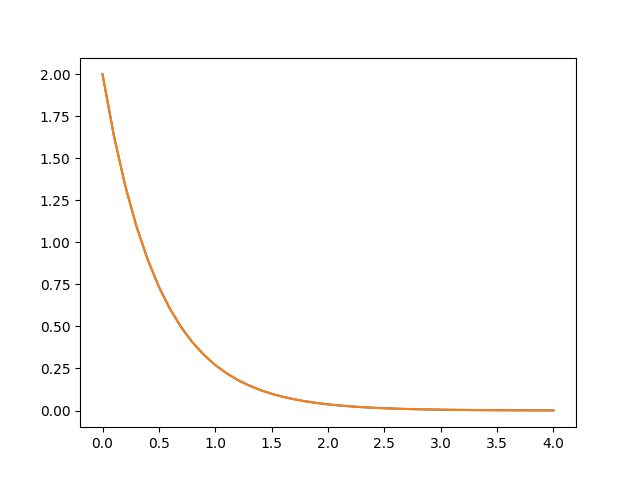
\includegraphics[totalheight=8cm]{figure-1.png}
    \caption{График полученного графика 1}
\end{figure}

\begin{lstlisting}[
    language={Bash},
    caption={Результаты работы программы 2}
]
$ bash ci/run.sh < res/2.txt
=== Welcome to differential eqsolver ===

Here you can solve differential equations using:
- Basic Euler
- Corrected Euler
- Runge-Kutta 4
- Milne

Choice a one of first-order equations:
[0]: dy/dx = y + (1 + x) * y ^ 2
[1]: dy/dx = -2 * y
[2]: dy/dx = 2 * x * exp(x ** 2) / (exp(x ** 2) + 1)
Enter a number of equation i in [0..2]: Taken: dy/dx = 2 * x * exp(x ** 2) / (exp(x ** 2) + 1)
Enter boundaties: 
Enter x_0: Enter y_0: Enter x_n: Enter h: Enter eps: 
Input parameters: 
> x_0 = 0.0
> y_0 = 0.69314718056
> x_n = 4.0
> h   = 0.1
> eps = 0.001

Enjoy results!

=== Report of Basic Euler === 

Result of Basic Euler is 15.99181773714573
Total iterations: 11239
Stop at: 3.999999999998924

=== Report of Corrected Euler === 

Result of Corrected Euler is 16.00001130507996
Total iterations: 3524
Stop at: 4.000000000000414

=== Report of Runge-Kutta 4 === 

Result of Runge-Kutta 4 is 16.00000010821849
Total iterations: 737
Stop at: 3.9999999999999227
\end{lstlisting}

\begin{figure}[h]
    \centering
    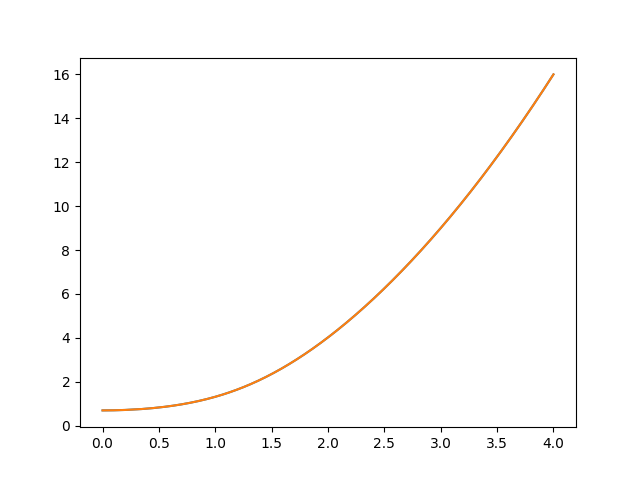
\includegraphics[totalheight=8cm]{figure-2.png}
    \caption{График полученного графика 2}
\end{figure}

\section{Вывод}

Выполнив данную лабораторную я познакомился с
базовыми методами решения дифференциальных уравнений.
Точность методов контролировалась правилом Рунге.
Метод Эйлера гораздо менее эффективнее, чем метод
Рунге-Кутта, что и ожадалось, ведь точность первого
метода $O(n)$, а второго аж $O(n^4)$. Графики при 
малых шагах на глаз совпали с дейтсвительными ответами.

\begin{thebibliography}{9}

    \bibitem{itmo-lecture}
    Лекции Татьяны Алексеевны Малышевой

\end{thebibliography}

\end{document}